\documentclass[12pt]{jreport}
\usepackage[dvipdfmx]{graphicx}
\input{jdummy.def}
%卒論用スタイルファイル
\usepackage{jgraduate2015_sjis}
%索引作成用
\usepackage{makeidx}
\usepackage{graphicx}
\usepackage{ascmac}
\usepackage{enumerate}
\usepackage{comment}
\usepackage{url}
\usepackage{cite}

% 前設定
\date{平成27年2月}
\title{WLANとZigBeeの共存に向けた\\AP-Assisted CTS-Blockingに関する研究}
\author{佐伯 良光}
\university{九州大学大学院}
\department{システム情報科学府}
\course{修士課程}
\major{情報知能工学専攻}
\subcourse{社会情報システム工学コース}

\begin{document}
%表紙
\maketitle

\begin{abstract}
% 概要
現代社会において,無線ネットワークによる通信は生活に不可欠な存在である.
特に近年,無線LAN(Wireless LAN,WLAN)通信はモバイル端末の普及などの要因も
あり,広く一般に利用されている.
%スマートフォンの登場によりWi-fiに代表される
一方,別のネットワーク通信としてZigBeeが注目されている.
ZigBee端末は他の無線ネットワーク端末に比べ安価で省電力であるため,
%例えば,ZigBeeネットワーク接続されたセンサを配置し
%電力やガスの消費量,温度を最適に自動制御するスマートハウス
%といった
センサネットワークを用いたM2M(Machine to Machine)技術に利用される.
しかしながら,WLANとZigBeeでは同一の周波数帯を利用するため,
干渉が発生し通信が阻害されるため共存が難しい.
そこで,同一周波数帯を利用するWLANとZigBeeの共存に向けて
容易に構築可能な衝突回避方式の研究を行っている.
衝突回避方式の実現に向けては既存の機器をそのまま利用できることが必要となることから,
OSやハードウェアの改変を必要としないシンプルな方式の実現が重要となる.
%衝突回避方式においては通信の公平性確保の目的で,システム改変に多くの制約があるため,
%このような観点から,既存の方式を活用する,フレームを二重に送信する等,システム改変の
%これらの制約にあたらないシンプルなシステム構築が重要となる.
本論文ではこのような観点で設計された
AP-Assisted CTS-Blocking(AA CTS-Blocking)方式を示す.
AA CTS-Blocking方式ではRTS/CTS方式を応用することでWLANの通信を抑制し,ZigBee通信と
WLAN通信の衝突を回避させる.
RTS/CTS方式はWLANの標準に定められた衝突回避機構であり,所定の手順を踏んで
RTS/CTSフレームを送信することでOSやハードウェアの改変を行うことなく
WLANとZigBeeの衝突を抑制することができる.
AA CTS-Blocking方式を適用したZigBeeデータ収集システムを実装し,
実証評価を通じてAA CTS-Blocking方式の衝突回避効果により
ZigBee通信の成功率が向上したことを確認した.


\end{abstract}


%目次
\tableofcontents

\newpage

%ページ番号をアラビア数字に
\pagenumbering{arabic}


\chapter{はじめに}\label{intro}%==============================================
%WLAN利用例を示し,WLANが普及していることを示す.分量もう少し増やす(後ほど)
現代社会において,無線ネットワークによる通信は生活に不可欠な存在である.
特に近年,無線LAN(Wireless LAN,WLAN)通信はWi-FI等で広く一般に普及している.
例えばPCとプリンタを,自宅のWLANアクセスポイント(Access Point,AP)に接続し
印刷を行うことは珍しくない.
それだけにとどまらず,更にHDD,テレビ,レコーダーなど,様々なデジタル機器を
WLANネットワークに接続して利用するホームネットワークという概念も登場している.
近年では,WLAN通信端末の主体がスマートフォンやタブレットで代表される
モバイルワイヤレス端末に移行しつつある.
コンビニエンスストアや駅など,不特定多数の人々がゲストとしてアクセス可能な
WLAN APの設置も進んでいる.
特定の場所に限らず,あらゆる地域・場所でWLANネットワークに
接続して通信することが求められるようになってきている.

%ZigBee利用例を示し,ZigBeeがこれから増えていくことを示す.分量もう少し増やす(後ほど)
他方で,別のネットワーク通信としてZigBeeが注目されている.
ZigBeeとは,IEEE 802.15.4に準拠したセンサーネットワークを主目的とする
近距離無線通信規格の1つであり,WLANに比べ通信距離が短く通信速度も
低速であるが,安価で省電力である.
それ故に,ネットワークに繋がれた機器同士が人間を介在せずに通信し,
サービスを提供するM2M(Machine to Machine)技術によく利用される.
M2Mの応用範囲は非常に幅広く,多様なサービスを提供可能である.
屋内にZigBeeネットワーク接続されたセンサを配置して,
電力やガスの消費量や,温度を最適に自動制御するスマートハウスもM2Mの1つである.

%干渉の話分量もう少し増やす(後ほど)
ネットワーク技術の進歩に伴い人々の暮らしが益々便利になる
一方で,通信フレームの衝突による干渉という課題も存在する.
例えば,ZigBeeセンサにより構築されたスマートハウスを利用する場合,
屋内にWLAN APが存在すれば干渉が発生する可能性は高い.
干渉とは,電波技術Aに対応した受信機Txが電波Aと電波Bの混在した電波を受信した際,
正常に電波をデコードできないことを指す.
これはZigBeeが,WLANと同じ2.4GHz帯を利用するためである.
図\ref{fig:frequency}に,WLAN及びZigBeeの周波数チャネルを示す.
ZigBeeのすべてのチャネルはWLANの複数のチャネルと重なっており,
ZigBeeとWLANの中心周波数が近いところでは相互に干渉が生じる
ことが報告されている~\cite{shuaib06:wifi_zigbee}.
WLANはZigBeeに比べて10〜100倍程度送信電力が大きいため,
干渉による通信への影響はZigBee側が大きい.

\begin{figure}[bt]
 \centering
 \includegraphics[width=\columnwidth]{figure/frequency.pdf}
 \caption{WLAN及びZigBeeの周波数チャネル}
 \label{fig:frequency}
\end{figure}

WLAN,ZigBeeにはアクセス制御方式としてCSMA/CA
(Carrier Sense Multiple Access / Collision Avoidance)機構を具備している.
しかし,WLANのCSMA/CAではWLANのみの通信環境,
ZigBeeのCSMA/CAではZigBeeのみの通信環境を想定しているため,
%これはWLANのみの通信環境,もしくはZigBeeのみの通信環境を想定しているため,
%従って,同種の通信における干渉回避を目的としている.%←合ってる?
%そのため,異種の通信におけるフレーム衝突回避を目的とした
WLAN通信とZigBee通信が混在した環境において互いの干渉を回避することは困難である.

WLAN通信とZigBee通信が混在した環境内におけるWLANとZigBeeの共存を目的とした干渉回避方式として,
文献~\cite{hou09:minimize_intf}ではWLANのアクセス制御であるRTS/CTS(Request to Send / Clear to Send)方式
を利用したCTS-Blockingが提案されている.
図\ref{fig:cts_blocking}に,CTS-Blockingの概要を示す.
CTS-Blockingでは,制御PCからCTSフレームを直接送信することで周囲の
WLAN端末の通信を一時的にブロックする.
WLAN通信において,送信端末以外の端末がCTSフレームを受信すると
CTSフレーム内の\texttt{Duration}フィールドに記載された時間だけ送信を控える.
CTS-Blockingではこれを利用して周囲のWLAN端末の
通信を抑制し,WLANとZigBeeの干渉を回避する.
しかしながら,現在のOS・無線LANモジュールでは通信の公平性確保の観点からCTS
フレームの直接送信が禁止されており,CTS-Blockingの実現に向けてハードウェアや
OSの改変が必須となる.
また,送信電力制御の影響によりCTSフレームの到達範囲が狭くなる可能性があり,隠れ端末問題の影響を受けやすい.

WLANとZigBeeの共存のためには,%WLANのアクセス制御を行うことで
%干渉されないZigBee通信を
ハードウェアやOSを改変することなく,
既存のモジュールをそのまま用いてWLANからの干渉を受けないZigBee通信を実現する
ことが重要である.
これに向け,筆者らは既存のRTS/CTS方式をそのまま利用した
%WLANのアクセス制御である
AP-Assisted CTS-Blocking(AA CTS-Blocking)干渉回避方式の開発を進めている.
本稿では,AA CTS-Blocking方式について述べ,その有効性の検証に向けた実証評価について報告する.

\begin{figure}[bt]
 \centering
 \includegraphics[width=\columnwidth]{figure/cts_blocking.pdf}
 \caption{CTS-Blockingと隠れ端末問題}
 \label{fig:cts_blocking}
\end{figure}

本論文の構成は以下の通りである.
\ref{fundamental}章ではWLAN及びZigBeeの基礎技術について触れ,アクセス制御方式などの説明を行う.
\ref{relation}章ではWLANとZigBeeの共存に向けた干渉回避方式に
関する研究について述べ,既存システムの課題を示す.
\ref{aa_cts}章では筆者らが提案するAA CTS-Blocking方式の概要及び設計について示す.
\ref{imple}章ではAA CTS-Blocking方式を適用した
ZigBeeノードによるデータ収集システムの実装について述べ,
\ref{eval}章でWLAN通信環境下におけるZigBeeノードによるデータ収集システムについて,
AA CTS-Blocking方式の有無による通信成功率の差を比較・考察する.
最後に\ref{conclu}章でまとめとする.

\chapter{WLAN及びZigBeeに関する基礎技術}\label{fundamental}%==============================================
本章では電波干渉の原因及び干渉回避方式について正確な知見を得るため,
WLAN及びZigBeeの基礎部分について簡単に説明し,利用されている
MACプロトコルなどについて説明する.\\

%以下で説明する技術には主に位置ベースの技術とメディアベースの技術とに大別される.\\

\begin{comment}
混信の問題で送・受信周波数と周波数帯域幅の関係が影響してきます。
大まかに言うと受信周波数帯に妨害電波(雑音)の関係で、
1.同一周波数で送信周波数が同じ複数の電波の場合(BさんとCさんは発信する)
1)AM変調波であれば、Aさんの受信する信号は混信します。
2)FM変調波であれば、BさんとCさんの信号でどちらか強い方がAさんは受信でき、弱い方は受信できません。

>ようは、同じ周波数で同時に通信を行うと、その複数の電波が交じり合って元々の信号が歪められる?ということでしょうか
同じ受信信号レベルであれば、そうなります。
AM変調波であっても、強力な受信信号レベルの方が、弱い受信信号レベルの方を抑圧します。

2.違う周波数でも影響を受ける場合
1)電子レンジの周波数帯は2.4GHz周波数帯で、無線LANに影響する場合
 電子レンジの占有周波数帯は広範囲に広がっており、無線LANの受信CHで妨害の程度が変わってきます。
2)送信信号が強力な場合(受信機が近くにある場合)
 受信機の入力段で歪み(混変調)を生じて、妨害を受け受信周波数以外を受信する場合があります。
3)送・受信周波数が隣接CHで混信する場合
 送・受信周波数が隣接CHの関係で混信し受信する場合があります。
4)送信側(ノイズ源)で、スプリアス電波成分が多数含まれている場合

>放射される電波の電界強度の違いでしょうか。
>極端な例ですが、電界強度が同等か、●●倍だと影響は受けるけど、1/2だと影響を受けないとか。
電波法で送・受信性能特性に規制があり、特に送信のスプリアス電波には2・3倍・・・・の他目的外の周波数成分発射には法規制値が定めてあります。
受信性能特性にも選択度や受信周波数帯域幅の規定があります。
*詳細部分は電波法を参照ください。

>同じ周波数で同時に通信を行うと、その複数の電波が交じり合って元々の信号が歪められる?ということでしょうか。

ちょっと違います。電波が交じり合っただけでは干渉しません。
\# 例えば指向性の鋭いビームアンテナがあれば、同じ周波数でもそれぞれの電波を明瞭に分離できます。
地球上ではには長波帯からマイクロ波帯まで様々な電波が飛び交っていますが、そうでなければ互いに干渉しあって、無線通信は使い物になりません。

干渉とは、受信した後の現象です。
無線通信機は、アンテナで電波を電流に変換した後、同調回路やフィルタで目的の周波数成分のみを取り出し、増幅、検波して信号成分を取り出し、更に増幅して、音声などの信号を外に出します。

同じ周波数の電波を同時に受信してしまうのは単なる混信であり、受信機にとっては正しい動作をしているものの、聞く人には何を言っているか分からなくなるだけです。
ようは、2人が同時にしゃべると、聖徳太子でない限り聞き分けられないのと同じです。
%まぁ、これも音声レペルの一種の干渉ですが。

問題は二番目の、違う周波数の電波による干渉で、これを混変調といい、増幅器の性能に大きく依存します。
理想的な増幅器は、入力と出力との関係がきれいな直線関係にあるものですが、一般には僅かに歪みがあり、これが様々な周波数成分を生み出します。
特に問題なのが三次の混変調と呼ばれるもので、目的の周波数f1と妨害調周波数f2を同時に受信したとき、mf1±nf2(m,nは整数)がf1に近いとき、フィルタでは取り除くことができず、混信となります。
一般にはこの成分は問題とはなりませんが、f2の強度が極めて大きいとき、強度の2乗で干渉してくるので、強い混信となります。
一時期問題となった、違法トラック無線などが良い例です。

尚、最近の携帯電話などはデジタル化され、無線機内で様々な信号処理をしているので、混信や混変調はほとんど問題となりません。
\end{comment}


\chapter{関連研究及びその比較}\label{relation}%==============================================
%筆者らの調査の範囲では
干渉回避方式に関する研究は膨大に存在するが,
大別すると
\begin{enumerate}

 \item WLAN/ZigBeeの既存のアクセス制御方式を利用した\\
 方式~\cite{hou09:minimize_intf,zhang11:zigbee_wifi_coexist,murata14:wlan_zigbee,huang09:wlan_zigbee,tytgat12:wlan_zigbee}
%~\cite{zhang11:zigbee_wifi_coexist}
%~\cite{murata14:wlan_zigbee}
%~\cite{huang09:wlan_zigbee}
%~\cite{tytgat12:wlan_zigbee}

 \item 既存のアクセス制御方式以外の技術を利用した
 方式~\cite{huang10:beyond_coexist,liang10:wifi_zigbee_survive}
 %~\cite{liang10:wifi_zigbee_survive}

\end{enumerate}
に分類される.
%本節ではこれらの研究について紹介を行う.

WLANのCSMA/CA機構を利用した干渉回避方式としてCBT~\cite{zhang11:zigbee_wifi_coexist}が挙げられる.
%CBT~\cite{Zhang11:},ACROS~\cite{Shin10:}においても同様の問題が考えられる.
CBTでは,
signalerと呼ばれるZigBeeノードをWLAN機器の近くに配置し,ZigBee通信時にsignalerから
長いフレームを送信することでWLAN端末にZigBeeが通信状態にあることを通知する.
WLAN端末ではsignalerの送信信号によりCSMA/CA機構が働き,送信が抑制されるため
WLANとZigBeeの衝突を回避できる.
%CBT(Co-operative Busy Tone)
%CSMA/CAを用いて,WLAN端末にZigBee通信が開始されることを知らせ
%ZigBeeノード間で通信が行われる間WLAN端末のデータ送信を控えさせることにより,
%WLANとZigBeeのフレーム衝突を回避する.
しかしながら,
スマートフォンなどの移動体も含めて考えると
全てのWLAN機器の近くにsignalerを配置することは非現実的である.
%構築には全WiFi端末の近くにsignalerと呼ばれるZigBeeノードを
%配置する必要があるため,モバイルWLAN端末に対して非現実的である.

また,
%WLANのアクセス制御方式である
%DCF(Distributed Coordination Function)を利用した干渉回避方式も提案されている.
村田ら~\cite{murata14:wlan_zigbee}は干渉の原因をZigBeeのaTurnaroundTime(送受反転時間)が
通信アイドル時の待機時間であるDIFS(DCF Inter Frame Space)よりも長いことと捉え,
DIFSを拡大する方式を提案している.
DIFSをaTurnaroundTimeに比べ長くとることで衝突を回避する.
しかしながら,DIFSを拡大するためには予めAPにアクセスして設定しなければならず,
%またDCFの欠点である,物理的障壁が存在した場合の隠れ端末問題の影響を考えると
実現のためには周囲のAP全てを管理下に置かなければならない.

ZigBeeが準拠しているIEEE 802.15.4のビーコンモードによるアクセス制御を利用した
干渉回避方式も提案されている~\cite{huang09:wlan_zigbee}.
Dynamic GTSでは,ビーコンモードの1つである
ZigBeeノードにGuaranteed Time Slot(GTS)を割当て優先的に通信できる期間CFP(Contention Free Period)
を利用し,このCFPを拡大することで衝突を回避する.
CFPの拡大は,GTSを動的に配置しそのビーコンを検知したWLAN端末が
CTSフレームを送信することで達成可能である.
しかしながら,\ref{sec:intro}で示したCTS-Blockingと同様に
ハードウェアやOSの改変が必須である点,
隠れ端末問題の影響を受けやすい点が問題である.
CACCA~\cite{tytgat12:wlan_zigbee}においても同様の問題が考えられる.

既存のアクセス制御方式以外の技術を利用した方式として,
%例として,WISE~\cite{Huang10:}及び
%BuzzBuzz~\cite{Chieh10:}を紹介する.
無線通信の通信空き時間を有効活用して通信を行うための「White Space」技術
を応用した干渉回避方式が提案されている~\cite{huang10:beyond_coexist}.
WISEでは,WLAN通信におけるWhite Spaceを予測し,そのWhite
Space内で通信が完了するようにZigBeeフレーム長の動的制御を行う.
例えば,WLAN通信の混雑時には予測されるWhite Spaceの長さは短くなるため,
ZigBeeノードにおいてデータを分割して送信する.
これにより,ZigBeeフレームがWLAN通信によって破壊される確率を低減させるこ
とが可能となる.
しかしながら,WLAN通信が混雑している時にはWLAN通信の空き時間が少ないため
にWhite Spaceの予測が外れ,通信が衝突する確率が高くなる.

フレーム衝突について分析し,分析結果を干渉回避方式とした研究もある.
BuzzBuzz~\cite{liang10:wifi_zigbee_survive}では,WLANとZigBeeのフレーム衝突により通信が阻害される原因として
IEEE 802.15.4フレームのヘッダが破壊されることと捉え,
ヘッダを2重にして送信することでZigBeeのパケットロス率を減少させている.
BuzzBuzzはこれまでに紹介した関連研究群とは違い,
%これまでに説明した関連研究群は,
既存の方式やモジュールの改造及び特別なハードウェア等の利用が必要なく,
干渉回避方式の構築コストについて考慮されている.
%既存の方式のみを利用した干渉回避方式に関する研究は報告が少なく,
%筆者らの調査の範囲ではBuzzBuzz~\cite{Chieh10:}が該当する.
これは,本稿で提案するAA CTS-Blocking方式とは違うアプローチで
ZigBeeの通信を保証しており,
%干渉回避方式として効果を上げている.
AA CTS-Blockingと組み合わせることでさらなる干渉回避効果が期待される.

%干渉回避方式に関する研究は膨大に存在するため,本節ではそれらについて俯瞰する.


%RTS/CTS方式を利用した干渉回避システムについても提案されている.
%図\ref{fig:cts_blocking}に,CTS-Blocking~\cite{Hou09:}の概要を示す.
%CTS-Blockingでは,制御PCからCTSフレームを直接送信することで周囲の
%WLAN端末の通信を一時的にブロックする.
%送信端末以外の端末がCTSフレームを受信すると,CTSフレーム内の\texttt{Duration}
%フィールドに記載された時間だけ送信を控える.
%CTS-Blockingではこれを利用して周囲のWLAN端末の通信を抑制し,WLANとZigBeeの
%干渉を回避する.
%この手法では単純にCTSフレームのみを利用しているため,
%WLAN通信の混雑度に左右されず,事前にAPへアクセスしてDIFSを設定する必要ない.
%これまで紹介してきた手法の中では,最も実環境における干渉回避効果が高いと期待できる.
%しかしながら,現在のOS・無線LANモジュールでは通信の公平性確保の観点からCTS
%フレームの直接送信が禁止されており,CTS-Blockingの実現に向けてハードウェアや
%OSの改変が必須となるために実現が難しい.
%また,送信電力制御の影響によりCTSフレームの到達範囲が狭くなる可能性があり,隠れ端末問題の影響を受けやすい.



%WLANとZigBeeの共存に向けて様々な手法,システムが提案されているが,
%その多くは複数のAPと自由なWLAN通信が行われる実環境に即していないように見受けられる.
%そこで筆者らは,実環境におけるWLAN及びZigBeeの干渉回避システムを目指し
%AP-Assisted CTS-Blockingを提案する.

%--------------------------------------------------

%----------------------------------------------------------------------
\chapter{AP-Assisted CTS-Blocking方式の提案}
\label{aa_cts}

WLAN APは,WLAN端末に比べ送信電力が
%物理的に
大きく,RTS/CTS制御方式においても利用されるため,
これを利用して干渉回避方式であるAP-Assisted(AA)
CTS-Blockingを提案する.
%本節では,AA CTS-Blockingの概要を示し,
%構築のための課題について検討する.

%APからCTSフレームを送信することはRTS/CTS制御方式において
%一般的であるため,OSやハードウェアの改変が不必要となる.
%またWLAN端末に比べ,WLAN APの送信電力が物理的に大きいことに着目し,
%AP-Assisted(AA)CTS-Blockingを提案する. 
%AA-CTS Blockingでは,周辺にあるWLAN APからCTSフレームを送信させてCTS-Blockingを実現する.
%かつ隠れ端末問題によるWLANフレーム衝突が改善され,ZigBee通信効率の向上が期待される.

\section{概要}
\label{sec:outline}

%これにより,WLAN通信の一時的ブロックによる効率的なZigBee通信の実現を目指す.
%また,RTSを送信するAPの選択については,APから取得できる情報を基に最適なAP選択アルゴリズムを考慮する.
図\ref{fig:aa_cts_blocking}に,AA CTS-Blocking方式の概要を示す.
本システムは,環境内に配置された複数のZigBee End Device(ZED)及び
ZigBeeネットワーク制御を行うZigBee Coordinator(ZC),制御PCから構成される.
ZigBee基地局と制御PCは有線接続されている.
AA-CTS Blockingでは,周辺にあるWLAN APからCTSフレームを送信させることでWLAN通信をブロックし
干渉の影響を低減したZigBeeノード間の通信を実現する.

%ZigBeeの通信を開始する場合,周囲のAPの1つを選択して制御PCからRTSフレームを送信する.
%選択されたAPはRTSフレームを受信すると周囲のWLAN端末に対してCTSフレームを送信する.
%制御PCはAPからのCTSフレームを受信するとZCを用いて複数のZEDとの通信を開始する.
%WLAN APは,そのAPが提供するWLANネットワークに参加していない端末からのRTSフレームに対しても
%CTSフレームを返答するため,制御PCでは任意のAPを選択することができる.

\begin{figure}[bt]
 \centering
 \includegraphics[width=\columnwidth]{figure/aa_cts_blocking.pdf}
 \caption{AA CTS-Blocking}
 \label{fig:aa_cts_blocking}
\end{figure}

\figurename~\ref{fig:sequence}にAA CTS-blocking方式の
通信シーケンスを示す.
制御PCは,あらかじめ周囲に存在するWLAN APのビーコンフレームを受信し,
チャネル,受信信号強度(RSSI)等を収集しておく.
ZigBeeノード間の通信を行う場合,まず(1)~制御PCはAPを1つ選択し,
(2)~制御PCは選択したAPに向けてRTSフレームを送信する.
次に(3)~RTSフレームを受信したAPは
周囲のWLAN端末に向けCTSフレームをブロードキャストする.
CTSフレームを受信したWLAN端末はCTSフレーム内の\texttt{Duration}
フィールドに記載された時間だけ送信を控えるため,WLAN通信が一時的にブロックされる.
WLAN通信ブロック期間がスタートした時,
(4)~CTSフレームを受信した制御PCは,有線接続されたZCに向けて通信開始信号を送信することで
ZigBeeノード間の通信を開始する準備が整う.
ZigBeeノード間の通信は
ZCを用いた制御によりWLAN通信ブロック期間内に完了させる.

このようなAA CTS-Blockingを実現する上では2つの疑問が生じる.
\begin{enumerate}
 \item RTS送信先APをどのように選ぶか
 
	実環境には多くのWLAN APが存在するため,
	制御PCはRTSの送信先APを選択する必要がある.
	%APによるCTS-Blockingの効果は選択するAPによって大きく異なるため,重要である.
	\ref{ssec:select_ap}において,周囲に存在するWLAN APのビーコンフレームを用いた
	AP選択アルゴリズムを示す.

 \item WLAN通信ブロック期間において,ZigBeeノード間通信をどのようにスケジューリングするか
 
 	WLAN通信ブロック期間は有限であるため,
	%ZEDの数が多いほど通信回数が増え,時間的制約が厳しくなる.
	%ZigBeeノード間通信が増加しても,
	ZigBeeノード間で通信の衝突が起きないようアクセス制御を行う必要がある.
	%データ収集のZigBeeネットワークでは,ZCと複数のZEDによるスター型のネットワークトポロジーになる.
	%ZigBeeノード間通信でフレーム衝突が起きないよう,スケジューリングを行う必要がある.
	%AA CTS-BlockingではZigBee通信成功率の向上を目的としているので,
	%WLANとZigBeeの干渉以外の事象に起因する通信失敗率の値を排除した
	%AA CTS-Blockingによる純粋なZigBee通信成功率の向上値を示すためにも重要である.
	\ref{ssec:design}において,1台のZCと複数のZEDとの通信における
	スケジューリング手法を検討する.

\end{enumerate}

\begin{figure}[bt]
 \centering
 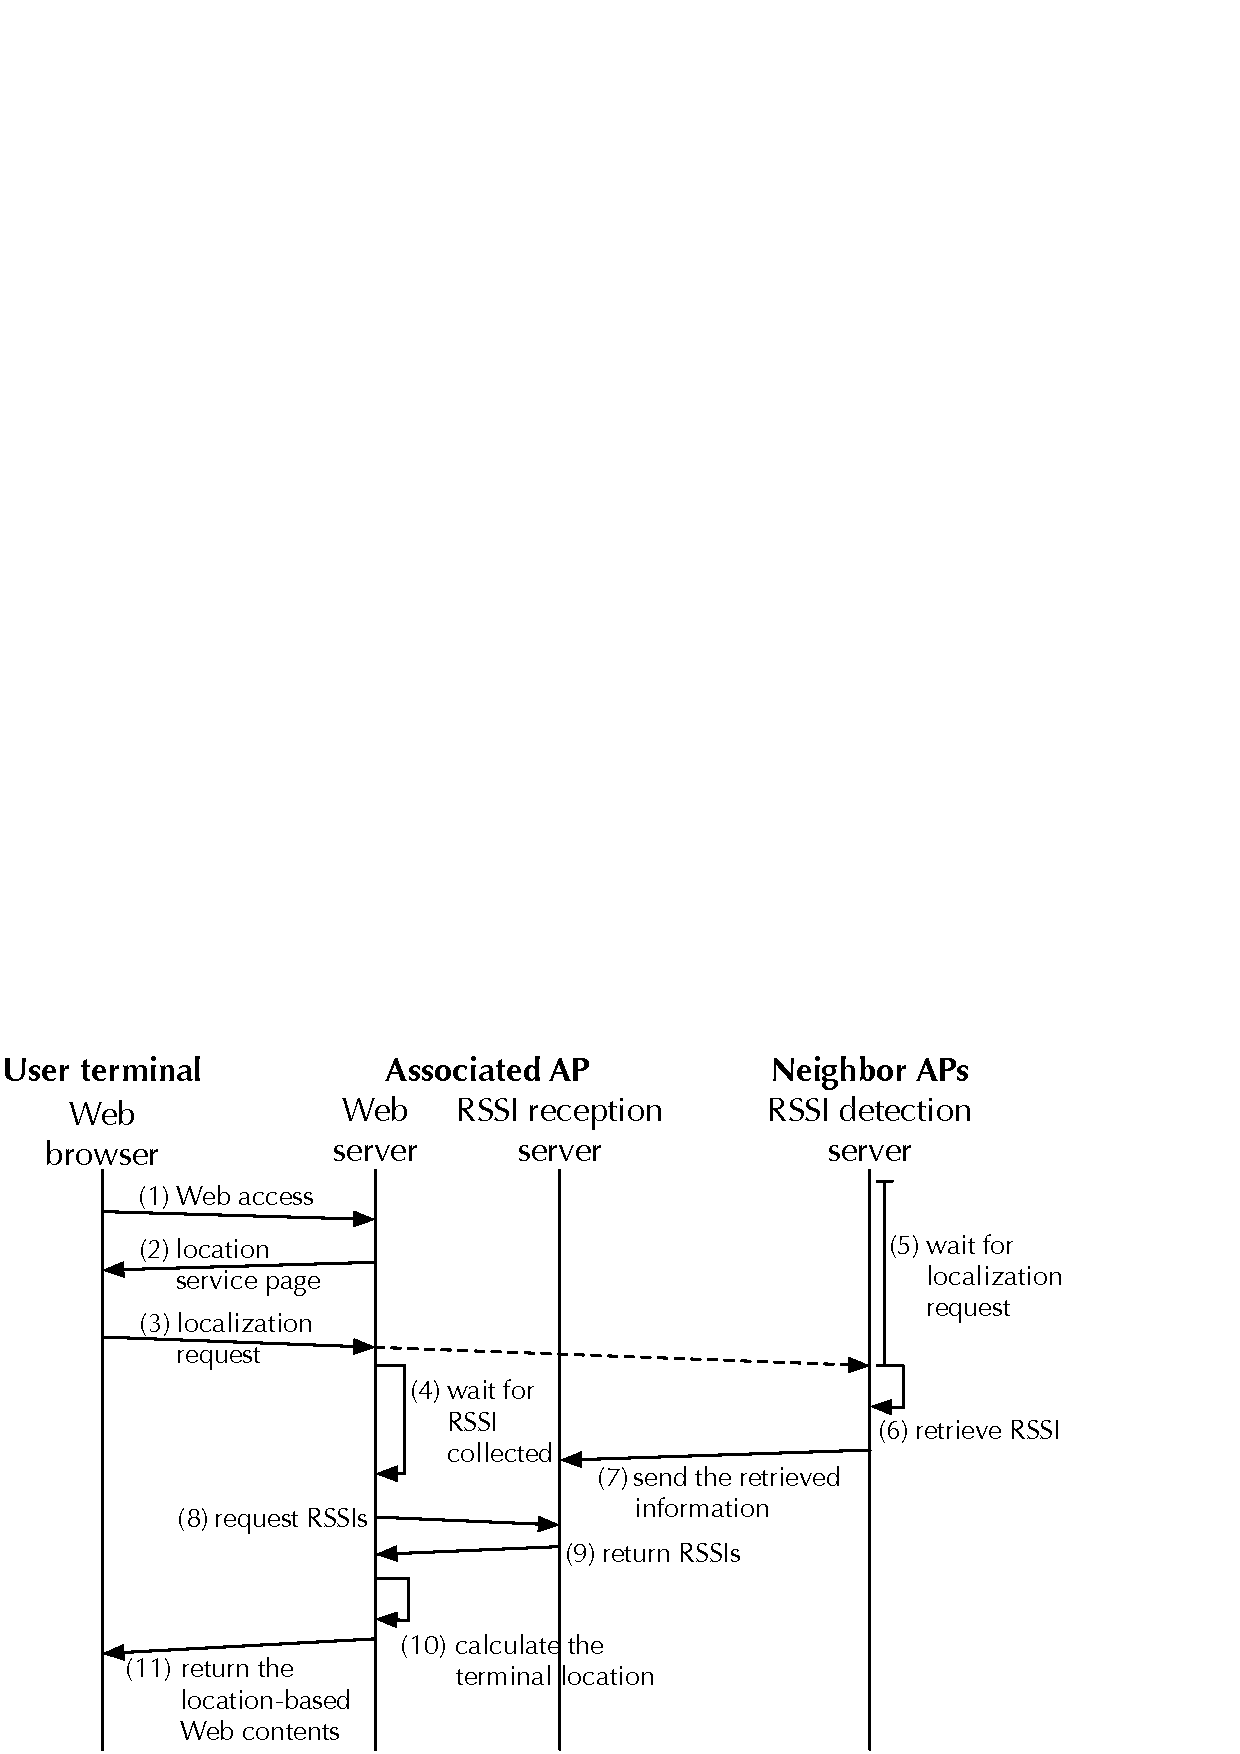
\includegraphics[width=\columnwidth]{figure/sequence.pdf}
 \caption{AA CTS-blocking方式の通信シーケンス}
 \label{fig:sequence}
\end{figure}

\section{AP選択アルゴリズム}
\label{ssec:select_ap}

AA CTS-Blockingにおいては,RTSフレームの送信先APの選択は
干渉回避性能に大きな影響を及ぼす.
例えば,制御PCの通信可能範囲ギリギリの位置に存在するAPを選択した場合
RTSフレームがAPに届かない可能性やAPからのCTSフレームを受信できない可能性がある.
%↓ここは情報が足りない
%あまり通信を行っていないAPを選択した場合
%わずかなWLAN端末の通信しかブロックできず本システムによる効果が薄い.
RTSフレーム送信先APの選択を最適化することにより,
より確実により多くのWLAN通信をブロックできる.
%× なぜならば,RTSフレームが制御PCの通信可能範囲にある必要がある
%○ 淡々と述べる
%制御PCとZCは一体になっている
%→データ収集システムにおいて,ZEDはZCを中心に周囲に配置されたものだとすると,
%RSSIによるWLAN通信のブロックはものすごく有効

本研究ではAPと制御PCの物理的距離が重要になると考え,
位置推定~\cite{izumi13:awpn_acc_imprv}などにも用いられる
RSSIをAP選択アルゴリズムのキーとして採用した.
RSSIの取得は特殊なパラメータや追加のデバイスを必要とせず,
%AP選択アルゴリズムに使用できる情報は,
既存のAPから発せられるWLANフレームを受信するだけで収集可能である.
図\ref{fig:aa_cts_blocking}に示すように制御PCがZCに有線接続されており,
ZEDはZCを中心に周囲に配置されていることも考慮に入れると,
制御PC周辺のWLAN通信をブロックすることが非常に有効であると考えられる.
%最も近いAPを選択することは非常に有効である.
%RSSIによるWLAN通信のブロックはものすごく有効
%ここで,本システムが有効であるためには
%制御PCの通信可能範囲にAPが存在する必要がある.
%従って,APと制御PCの物理的距離が重要になると考えられるため
%位置推定~\cite{izumi13:}などにも用いられるRSSIをAP選択アルゴリズムのキーとして採用した.
%具体的には,RTSフレームの送信先APとしてRSSIがもっとも大きいAPを
%選択するものとした.

\section{スケジューリング手法}
\label{sec:design}

%APから周囲のWLAN端末にCTSフレームが送信されると,
%ブロック時間はCTSフレーム内の\texttt{Duration}フィールドに記載された時間に等しい.
%マルチキャストなZigBeeノード間通信において,フレーム衝突を防ぐための
%スケジューリングは重要である.
AA CTS-Blocking方式においては,ZigBeeノード間の通信はAPから送信されたCTSフレーム内の
\texttt{Duration}フィールド(最大値は32\,ms~\cite{IEEE802_11-2007})に記載された時間内に終了させる
必要がある.
ZEDの台数が増えた場合通信回数が増え,1回のRTS/CTS送信での通信が難しくなるため,
スケジューリング等のアクセス制御方式が必須となる.

これに向け,本研究では既存のMACプロトコルを利用する.
MACプロトコルは種類を問わず利用可能である.
%32\,ms~程度ではあるが一定の通信時間を確保できるためである.
ZEDの台数が32\,ms間で通信できない台数に増加した場合には,
ZEDをグループ化し,ZCからの制御によってRTS/CTSの1回の送信に
対して1グループに通信を許可すれば良い.
ただし,グループ間での通信に関しては問題が残る.
これについては今後の研究課題とする.
%にノード番号を与え通信タイミングを制御することで
%フレーム衝突は大幅に減少すると考えられる.
%このスケジューリングに関しては,
%MACプロトコルの種類は問わず,どの手法でも適用可能である.

%AA CTS-Blocking方式ではZigBeeノードを用いたデータ収集システムへの適用を想定しており,
%使用環境としてはWLANとZigBeeの干渉による影響が大きい,
%利用周波数帯の変わらない状況を想定している.
%\figurename~\ref{fig:star}に示す代表的なZigBeeネットワークトポロジーの中で最も低コストな,
%ZC1台にZED複数台をそれぞれ1対1で接続するスター型を採用すると考えると,
%ZCからZED方向の送信はブロードキャストであり,ZEDからZC方向の通信はシングルキャストとなる.
%シングルキャストでは,ZCに向けた異なるZEDからの
%データフレーム衝突を回避するスケジューリングが必要であるが.
%これはTDMA(Time Division Multiple Access,時分割多元接続)で十分である.

一例として,TDMA(Time Division Multiple Access)方式のMACプロトコルを利用する場合,
\ref{ssec:outline}で示したZigBeeノード間の通信シーケンス部分は以下のようにすれば良い.
制御PCから通信開始信号を受信したZCは,周囲のZEDへデータ要求フレームをブロードキャストする.
%各ZEDはTDMA方式に従うので,
データ要求フレームを受け取ったZEDは,
データ要求フレームをSlot同期信号としてTime Slotを用いたアクセス制御を開始し,
ZED毎にあらかじめ定められたSlotにおいてZCに対してデータフレームを送信する.
%ZED毎に定められたSlot Sizeの時間だけ待機する.
%Slot Sizeの時間が経過した後,ZEDはZCへデータフレームを送信する.

%AA CTS-blocking方式全体の通信シーケンスとして,\ref{ssec:outline}からの続きを考えることにする.
%例えば,スケジューリングとしてTDMA(Time Division Multiple Access,時分割多元接続)方式を利用した場合
%Zigbeeノード間の通信シーケンス部分は以下の様になる.
%(5)~通信開始信号を検出したZCは,周囲のZEDへデータ要求フレームをブロードキャストする.
%各ZEDはTDMA方式に従うので,
%(6)~データ要求フレームを受け取ったZEDは,ZED毎に固定されたスロットサイズの時間だけ待機する.
%スロットサイズの時間が経過した後,
%(7)~ZEDはZCへデータフレームを送信する.

%この様にすることで,WLANネットワーク環境下においても
%AA CTS-BlockingによるZigBeeデータ収集システムは実現可能である.

%----------------------------------------------------------------------
\chapter{設計及び実装}
\label{imple}

本章では,AA CTS-Blocking方式を適用したZigBeeノードによるデータ収集システムの
設計及び実装について述べる.
はじめに,ZigBeeノードによるデータ収集システムを構成するハードウェア及びOSについて触れ,
UMLを用いた設計について説明する.
その後,データ収集システムの実装について述べ,
制御PCによるAA CTS-Blocking方式の制御アプリケーション実装を説明する.

%\section{データ収集システムの実装}

\begin{comment}
\ref{sec:collecting_system}で作成したステートマシン図を基に,
ZigBeeノードによるデータ収集システムの実装を行う.
MICAzのプラットフォームとして利用したTinyOS上では
利用可能なイベント駆動型プログラミング言語はnesCという,C言語の拡張である.
nesCを利用し,データ収集システムの実装を行った.
nesCは一般的なプログラミング言語ではないため,次項でnesCの概念について説明し,
その後ZigBeeノード及びZigBee基地局への実装を説明する.
\end{comment}

\section{ハードウェア}

\subsection{ZED}

%本システムにおけるZEDは,環境内に配置され,データをZCへ送信する.
%データの信頼性の観点から,各ノードのフレーム送信を確実に成功させる仕組みが必要である.
%図\ref{fig:3_02}に示すように,各ノードに送信を待機させるスロット時間を設定し,フレーム衝突の回避を図ったり,
%衝突した場合に備えてタイムアウトを設定しデータを再送する手法などがある.

本システムにおけるZigBeeノードは日本国内で入手しやすく,センサノードとして一般的な
Crossbow社のMICAz MPR2600J~\cite{Product/crossbow:micaz}を用いた.
図\ref{fig:mpr2600j}にその外観を示す.
MICAzは無線機能,CPU,メモリ等を有したノード部分と各種センサを搭載したセンサ基板部分から構成されるセンサノードであり,
MPR2600J(RF周波数帯2405MHz~2480MHz)はChipcon CC2420,IEEE 802.15.4 準拠,Atmega128L マイクロコントローラと
統合されたZigBee対応無線周波数トランシーバを使用しており,最大約50mの通信を行うことができる.
安定動作電圧は3.3V,消費電流は通信時60mA,スリープ時20μAである.
電源は単三乾電池2本から供給可能である.
端の一方にはON/OFFスイッチが,もう一方にはアンテナが付属している.

\begin{figure}[bt]
 \centering
 \includegraphics[width=\columnwidth]{figure/mpr2600j.pdf}
 \caption{MICAz MPR2600J}
 \label{fig:mpr2600j}
\end{figure}

%MICAzにはNode IDが設定できる.
%AA CTS-Blocking方式ではZigBeeノードを用いたデータ収集システムへの適用を想定しており,
%使用環境としてはWLANとZigBeeの干渉による影響が大きい,
%利用周波数帯の変わらない状況を想定している.
%\figurename~\ref{fig:star}に示す代表的なZigBeeネットワークトポロジーの中で最も低コストな,
%ZC1台にZED複数台をそれぞれ1対1で接続するスター型を採用すると考えると,
%ZCからZED方向の送信はブロードキャストであり,ZEDからZC方向の通信はシングルキャストとなる.
%シングルキャストでは,ZCに向けた異なるZEDからの
%データフレーム衝突を回避するスケジューリングが必要であるが.
%これはTDMA(Time Division Multiple Access,時分割多元接続)で十分である.
%上記データ収集システムのノード


%図\ref{fig:??}にその外観を示す.
%MICAzは
%無線機能,CPU,メモリ等を有したノード部分と各種センサを搭載したセンサ基板部分から構成されるセンサノードであり,
%最大約50mの通信を行うことが可能であり,
%安定動作電圧は3.3V,消費電流は通信時60mA,スリープ時20μAである.
%電源は単三乾電池2本から供給可能である.
%接続基板は
%本システムにおけるZCは,前述したZEDで使用するMICAzと,
%MICAzに対応したCrossbow社のMIB520~\cite{Device:}を用いた.
%I/OインターフェースとしてUSB Aタイプ(オス)を備え,電源はUSB バスを通じてPC から供給する.
%また,出力コンソールとして3色(赤,緑,黄)のLEDを利用できる.
%メス−メスUSB A-Aコネクタ(オス - メス)を用いてMICAz をMIB520 に装着し,制御PCと接続を行った.
%また,MIB520はオンボードでISP(in-system programming)に対応しており,
%シリアル通信及びシステムプログラミングを可能とする.
%但し,

%ノードへのアプリケーション実装は,PCで行った. 
%但し,PCにはTinyOS がインストールされていることが必要条件である.
%TinyOSはオープンソースで開発がされているセンサネットワークノード向けのイベント駆動OSであり,
%これを用いてZED及びZCのZigBee通信アプリケーションを実装した.
%TinyOS上で利用されるイベント駆動型プログラミング言語がnesCであり,C言語の拡張である.

%制御PCはDebian GNU/Linuxの動作するdynabook UX/28LWHEMを用いた.

\subsection{ZC}

%本システムにおけるZigBee基地局は,周囲のZigBeeノードからデータを収集し出力する.
%基地局は同一の周波数帯域内で2つ以上の複数の通信を行う多元接続方式の採用が必要である.
%そこでデータ収集として,図\ref{fig:3_04}に示すFDMA方式,TDMA方式,CDMA方式から最適な方式を選択する.
%データの出力については,基地局はPCに有線接続されているため,収集したデータをPCのコンソールに行うことが可能である.

本システムにおけるZCは,前述したZEDで使用するMICAzと,
MICAzに対応したCrossbow社のMIB520~\cite{Device:}を用いた.
図\ref{fig:zc}にその外観を示す.
I/OインターフェースとしてUSB Aタイプ(オス)を備え,電源はUSB バスを通じてPC から供給する.
また,出力コンソールとして3色(赤,緑,黄)のLEDを利用できる.
メス−メスUSB A-Aコネクタ(オス - メス)を用いてMICAz をMIB520 に装着し,制御PCと接続を行った.
また,MIB520はオンボードでISP(in-system programming)に対応しており,
シリアル通信及びシステムプログラミングを可能とする.
%但し,MOTE にプログラムするにはホストPC にTinyOS がインストールされていることが必要条件である.
メス−メスUSB A-Aコネクタ(オス - メス)を用い制御PCと接続して使用した.

\begin{figure}[bt]
 \centering
 \includegraphics[width=0.5\textwidth]{figure/zc.pdf}
 \caption{ZC(MICAz MPR2600J + MIB520)}
 \label{fig:zc}
\end{figure}

\subsection{制御PC}

%本システムにおける制御PCは,周囲のWLAN APに向けてRTSフレームを送信し,
%返ってきたCTSフレームの受信をトリガーとして有線接続されたZigBee基地局へ信号を送信する.
%APの選択アルゴリズムは,APから取得できる情報のみを基準にする必要がある.
%RTSフレームは通常,直接送信はできないため,擬似フレームとした.

制御PCはAA CTS-Blockingを動作させるため,
Debian GNU/Linuxの動作するdynabook UX/28LWHEMを用いた.
MIB520のI/OインターフェースはUSB Aタイプ(オス)であるため,
制御PCはメス−メスUSB A-Aコネクタ(オス - メス)を用いてZCと接続した.

\section{ZigBeeノードによるデータ収集システムの設計}
\label{sec:collecting_system}

データ収集システムの概要を図\ref{fig:aacts_snw}に示す.
%本システムでは,代表的なZigBeeネットワークトポロジーの中でも最も低コストな,スター型を採用した.
ZCを中心とするスタートポロジのネットワークを構築し,各ZEDからZCにデータを収集する.
WLAN通信ブロック期間におけるZigBeeノード間の通信はTDMA方式のスケジューリングを行い,
%ZEDのスケジューリングとしてTDMA方式を採用し,
各ZED毎に定められたTime Slotを設けた.
Time SlotはZEDのNode IDと対応付けており,
最大のTime SlotでもWLAN通信ブロック期間を超えないように定めた.
%ZC及びZEDには予めNode IDを設定しておく.
%ZCのNode IDはZEDの送信先アドレス,
%ZEDのNode IDはTime Slotに対応付けている.
%以下にデータ収集システムの動作を示す.
%\ref{ssec:outline}で示した通り,

制御PCから通信開始信号を検出したZCは周囲のZEDに向けてBroadcast Frame(BF)を送信する.
BFを受信したZEDは,BFをSlot同期信号として
ZED毎に定められたTime Slotに従い,Slot Sizeの時間だけ待機する.
Slot Sizeの時間が経過した後,ZEDはZCのNode IDを送信先アドレスとして
Unicast Frame(UF)を送信する.
%ZCが各ZEDへBFを送信することで通信を開始し,
%各ZEDがZCへUFを送信することでデータ収集が実施される.
%,待機後にZCへ送信した.
%Time SlotのSlot SizeはNode IDに比例する様に設定した.
%また,ZCのデータ収集実施時間はWLAN通信ブロック期間に等しく,
%この間は常に受信待機状態となるようにした.

\begin{figure}[bt]
 \centering
 \includegraphics[width=\columnwidth]{figure/aacts_snw.pdf}
 \caption{ZigBeeノードによるデータ収集システム}
 \label{fig:aacts_snw}
\end{figure}

%データ収集システムではZED,ZCにMICAzを利用したが,
ZED,ZCに利用したMICAzにおいて,ユーザーが定義可能なアプリケーション層の実装は
センサネットワークノード向けのイベント駆動OSとしてオープンソースで開発されているTinyOSを用いた.
TinyOSにおける実装はnesCによるイベント駆動型プログラミングとなり,C言語の拡張である.
%TinyOS上では
%利用可能なイベント駆動型プログラミング言語は
%nesCを利用し,データ収集システムの実装を行った.
nesCは一般的なプログラミング言語ではないため,\ref{ssec:nesC}項でnesCの概念について説明を行う.
%その後ZigBeeノード及びZigBee基地局への実装を説明する.
%イベント駆動型プログラミングでは,起動すると共にイベントを待機し,起こったイベントに従って処理を行う.
%イベントとは,プログラムの実行に際し,データを受信した,起動していたタイマが完了した等,
%何らかのアクションが発生した際にプログラムに発信される信号である.
%イベントを待機している間,MICAzは何らかの状態を持つ.
%このような状態遷移のフローをを記述するのに最適なのが,UMLのステートマシン図である.
%UML(Unified Modeling Language)は,抽象化したシステムをグラフィカルな記述でモデル化し,
%汎用的なプログラム設計図を与える.\\
%UMLで表現されるモデルには,システム実装を補助するために多くのダイアグラムが存在する.
%データ収集システムの設計では,システムを構成するZED,ZCの状態遷移を記述するためにステートマシン図を利用した.
%加えて,システム全体の流れを把握するためにシーケンス図を利用した.

\subsection{nesC}
\label{ssec:nesC}
%\subsubsection{TinyOS,nesC}

本節ではnesCの基本概念について,簡単なチュートリアルを交えながら説明する.

\begin{itemize}

 \item[1.] コンポーネント(component)
 
 コンポーネントとは,カプセル化されたソフトウェアの部品であり,同等の機能をもつものと交換可能である.
 nesCにおいて,アプリケーションのプログラムはコンポーネントで作られ,その組み合わせによりプログラム全体が形成される.
 コンポーネントは2つのスコープ(ある変数や関数が特定の名前で参照される範囲)を定義する.
 1つはコンポーネントの規定部スコープ(コンポーネントのインタフェースインスタンスの名前を含む)であり,もう1つはコンポーネントの実装部スコープである.
 コンポーネントはタスク(task)という形によって内部的に並列動作性を持つ.
 制御の流れはコンポーネントのインタフェースを通じて他のコンポーネントへと流れる.
 これらの制御の流れはタスクやハードウェア割り込みから生じている.
 
 \item[2.] インタフェース(interface)

 一連のインタフェース(interface)によるコンポーネントの動作の規定
      \item インタフェースはコンポーネントによって提供(provide)されるか利用(use)される.
      \item 提供インタフェースは、コンポーネントがそのユーザに提供する機能をあらわす.
      \item 利用インタフェースはコンポーネントが処理を行うために必要とする機能をあらわしている.
     \end{itemize}
  %\item インタフェースは双方向性を持つ
    \begin{itemize}
      \item インタフェースはインタフェースの提供者が実装すべき関数群(コマンド)とインタフェースの利用者が実装すべき関数群(イベント)を示す.
      \item これにより一つのインタフェースでコンポーネント間の複雑なやりとりを表現することができる(例えば興味のあるイベントに登録しておけば、そのイベントが起こったときにコールバックされる).
      \item TinyOS ではすべての時間のかかる処理(例:パケット送信)はノンブロッキングであるため,このことは重要である.時間のかかる処理の完了はイベント(例:送信完了)を通じて知らされる.
      \item 概してコマンドは呼び下げ,すなわちアプリケーションコンポーネントからハードウエアに近いところへ向かって順に呼ばれていく.一方,イベントは呼び上げられていく.
      \item いくつかの低レベルイベントはハードウエア割り込みに結びつけられている(どのように結びつけられるかは基本的にはシステム依存である).
     \end{itemize}
   %\item コンポーネントはインタフェースを通じて互いに静的にリンクされる.
      \begin{itemize}
   	\item これは実行時の効率を向上させ,堅牢性を増し,プログラムのよりよい静的解析を可能とする.
       \end{itemize}
   %\item nesC はコードがすべてコンパイラによって生成されるようにデザインされている.
      \begin{itemize}
   	\item これによってよりよいコード生成と解析が可能となる.例として ,nesC のコンパイル時のデータ競合検出があげられる.
       \end{itemize}
   %\item  nesCの並列処理モデルは処理完了まで走りきる(run-to-completion)タスクと割り込みハンドラに基づいている.
      \begin{itemize}
   	\item 割り込みハンドラはタスクや他の割り込みハンドラに割り込むことができる.
	\item nesC コンパイラは割り込みハンドラが起こしうる潜在的なデータ競合を通知してくれる.
       \end{itemize}
  
  %\end{itemize}

\subsection{ステートマシン図}
ステートマシン図は無償UMLモデリングツールであるastah* communityを利用して作成した.
ステートマシン図の遷移は矢印で表されており,
説明はイベント[ガード条件]/アクションで記述される.
ガード条件は直前に発生したイベントの評価をするための条件である.
評価値は真もしくは偽の値を持ち,ガード条件に対して真であるときのみ遷移が許される.
アクションは遷移が起こると同時に実行される動作である.
以下で,各機器毎に詳細を説明する.
%\subsection{ZED}

ステートマシン図は状態と状態遷移によって表されることを前項で説明した.
状態をSn(nは添字),イベントをEn,ガード条件をGn,アクションをAnと表記し
ZCの状態遷移を考慮すると,
以下の通りになる.

\begin{itemize}
 \item S1:受信待機状態
 \item E1:ZCから送信要求フレームを受信する
 \item G1:送信要求フレームの受信成功
 \item A1:スロット時間待機するためのタイマを起動する
 \item S2:送信準備状態
 \item E2:タイマが終了する
 \item A2:データを送信する
 \item S3:送信完了状態
 \item A3:タイマをリセットする
\end{itemize}

AA CTS-Blocking方式によりZigBee通信を保証する時間は,\ref{sec:outline}で示したWLAN通信ブロック期間に等しい.
この時間はわずかであり,送信失敗した場合にタイムアウトによる再送の仕組みを設ける余裕が無い.
従って,送信成功かどうかの判定は行わない.
これらを総合すると,ZigBeeノードのステートマシン図は
図\ref{fig:zed_state}の様に描画できる. \\

\begin{figure}[bt]
 \centering
 \includegraphics[width=\columnwidth]{figure/zed_state.pdf}
 \caption{ZEDのステートマシン図}
 \label{fig:zed_state}
\end{figure}

%\subsection{ZC}
次に,ZCのステートマシン図を考える.
ZEDの場合と同様に,
状態をSn,イベントをEn,ガード条件をGn,アクションをAnと表記し
ZCの状態遷移を考慮すると,以下の通りになる.

\begin{itemize}
 \item S1:シリアル信号待機状態
 \item E1:制御PCから信号を受信する
 \item G1:信号の受信成功
 \item A1:DF測定のためのタイマを起動
 \item S2:ブロードキャスト準備状態
 \item A2:ZigBeeノードへブロードキャストする
 \item S3:受信待機状態
 \item E3:ZCへ
 \item G3:データの受信成功
 \item A3:コンソールにデータを表示する
 \item S4:受信完了状態
 \item E3',E4':タイマが完了する
 \item A3',A4':タイマをリセットする
\end{itemize}

ZEDと同様送信失敗した場合にタイムアウトによる再送の仕組みを設ける余裕が無いため,
S3状態はS2状態からA2の動作を伴い自動遷移するようにした.
他方で,S4状態に遷移した後,他のノードからのデータを受信して表示する必要がある.
そのため,S4状態に入った際すぐにS3状態へと自動遷移するようにした.
そして,A1で起動させたタイマが終了した際は,S3/S4状態に関わらずS1状態に遷移する事とした.
これらを総合すると,ZigBee基地局のステートマシン図は図\ref{fig:zc_state}の様に描画できる.

\begin{figure}[bt]
 \centering
 \includegraphics[width=\columnwidth]{figure/zc_state.pdf}
 \caption{ZCのステートマシン図}
 \label{fig:zc_state}
\end{figure}

\subsection{コンポーネント図}

前項で説明したnesCでは,

\begin{itemize}
 \item[$\clubsuit$]”プログラムは コンポーネントで作られ,コンポーネントによりプログラム全体が形作られるよう組み立てられる.”
\end{itemize}
   
とある.そこで,コンポーネント毎の機能を明確にするために
図\ref{fig:zed_compo},図\ref{fig:zc_compo}に示す,ZED及びZCにおけるコンポーネント図を作成した.
コンポーネント図とは〜なUMLダイアグラムであり,
〜

%\subsubsection{ZigBeeノード}

%\appendix programming_code

%\subsubsection{ZigBee基地局}

%\appendix programming_code

\begin{itemize}
 \item[$\clubsuit$]:シリアル信号待機状態
 \item E1:制御PCから信号を受信する
 \item G1:信号の受信成功
 \item A1:CTS-Blocking有効時間を測るためのタイマを起動する
 \item S2:ブロードキャスト準備状態
 \item A2:ZigBeeノードへブロードキャストする
 \item S3:受信待機状態
 \item E3:ZigBeeノードからデータを受信する
 \item G3:データの受信成功
 \item A3:コンソールにデータを表示する
 \item S4:受信完了状態
 \item E3',E4':タイマが完了する
 \item A3',A4':タイマをリセットする
\end{itemize}

\subsection{シーケンス図}

図\ref{fig:zigbeecomm_sequence}にデータ収集システムのシーケンス図を示す.
シーケンス図は,オブジェクト間の相互作用を時系列に沿って表現するUMLダイアグラムである.
シーケンス図での時間は,ライフラインに沿って上から下に進む.
ここでは,システム全体の処理の流れが確認できる.

\section{データ収集システムの実装}

\ref{sec:collecting_system}で作成したステートマシン図を基に,
ZigBeeノードによるデータ収集システムの実装を行う.

%--------------------------------------------------

%----------------------------------------------------------------------
\section{AA CTS-Blocking方式の実装}
\label{sec:aa_cts_imple}

AA CTS-Blocking方式の動作の実証と基本性能の評価に向け,
PC及びZigBeeノード用いて,AA CTS-Blockingを適用した
ZigBeeノードによるデータ収集システムを実装した.

AA CTS-blocking方式を実現する
制御アプリケーションはC言語で実装した.
モニターモードの無線LANインタフェースを用い,
libpcapライブラリを利用することで環境中に流れるフレームを
傍受し,RTS/CTSフレームのキャプチャを行う.
また,RTSフレームの送信にもlibpcapライブラリを利用した.
%及びZCとの通信を可能としている.

RSSIによるAP選択アルゴリズムにおいてもlibpcapライブラリを利用した.
制御アプリケーションの開始時に
Radiotapヘッダが付加されたIEEE\,802.11ビーコンフレームを1.5\,秒間収集した.
収集したフレームを解析し,RSSIがもっとも大きいAPをRTS送信先として選択した.

%ここで,WLANが準拠しているIEEE 802.11で策定されている,
%IEEE 802.11フレーム共通のMACフレーム(参考文献)を\ref{fig:mac_header}に示す.
%スニファにより取得したWLANフレームにおいて,
%MAC(Media Access Control)層で付加されるヘッダを利用する事でWLAN端末接続数の計算は可能である.
%MACヘッダの3〜5ユニット目を抜き出すと,
%Address 1(DA)及びSA,BSSIDがある.
%WLAN端末の通信はAPを介するため,BSSIDとDAまたはSAが一致する筈である.
%APのBSSIDは既知であるため,
%AP1台に対し,APのBSSIDがDAになる場合の相異なるSAは取得可能である.
%その逆も同様に可能である.
%従って,APのBSSIDがDAの場合のSA及び,APのBSSIDがSAの場合のDAの共通部分を取り,
%これをキーとしたテーブルをAP毎に作成する.
%テーブルの行数がAPのWLAN接続台数に等しいため,最も行数の多いAPを選択することが
%AP選択アルゴリズムの決定キーとなる.

%--------------------------------------------------

%----------------------------------------------------------------------
\chapter{評価}
\label{eval}

提案するAA CTS-Blocking方式の有効性を
検証するために評価実験を行った.
まず,予備実験を行ってデータ収集システムを動作させる
パラメータであるSlot Sizeを決定した.
%まず,未決定パラメータの最適値を探るため,
%\ref{sec:imple}で述べたTime SlotのSlot Sizeを決定するために,
%電波暗箱内で
%データ収集システムの予備実験を行った.
%全パラメータ決定後は,
次に,AA CTS-Blocking方式がWLANの混雑度に関わらず
高い干渉回避効果を有することを示すために,
ZigBee通信の成功率の評価を行った.

%評価の流れは書いて欲しい。何のために予備実験をして、
%それからどんな評価(項目のこと)をしているのかの情報が欲しい。

\section{予備実験}
\label{ssec:before_exp}

%電波暗箱内で
\ref{sec:imple}で述べたTime SlotのSlot Sizeを決定するために,
データ収集システムの予備実験を行った.
%予備実験は,他の電波の影響がない環境で
%データ収集システムの動作を評価する.
適切なSlot Size決定に向けては,ZigBeeノード間の通信を保証した上で
通信が失敗しないことを確認する必要があるため,
予備実験では電波暗箱内でデータ収集システムの動作を評価した.
%適切なSlot Sizeでない場合ZigBeeノード間の通信において
%ZigBeeフレーム同士が衝突する可能性があり,
%後の実験で正しく評価できない恐れがあるためである.
図\ref{fig:nowave_box}に,電波暗箱内に配置したデータ収集システムを示す
%まず,スロットサイズを決定するために他の電波による干渉がない場所で
%ZigBee通信のみを評価する.
ZigBeeノード間で送受信するデータは,サイズの変化による影響をなくすため
送信元アドレス及びシーケンス番号のみが記録されたダミーデータとした.
サイズはヘッダを含めて18バイトと一定である.
18バイトのデータ送信に要する時間は,
ZigBeeの公称通信速度250\,kbps~\cite{IEEE802_15_4-2006}から計算すると
0.576\,msである.

本システムにおけるSlot Sizeは,データの送信時間に加えて
MICAzが送受信の切り替えに要する時間及びガード時間を含めたものを想定している.
%採用するSlot SizeではZCのデータ収集率が100\%になるものを選択する必要がある.
ZCは全10台のZEDからダミーデータを収集する.
予備実験では
%異常値を排除するため,
データ収集の試行を200回行った.
\ref{sec:imple}で述べた通り,ZigBeeノード間の通信時間が最大32\,msであり,
データの送信時間が0.576\,msであることを考慮に入れ,
Slot Sizeを1\,ms〜3\,msで変化させながらデータ収集予備実験を行った.
%なぜSlot Sizeを1~3にしたのか
このときPacket snifferを用いてエラーパケットの有無を監視し,通信成功台数を測定した.
通信成功台数とは,1回のデータ収集試行でZEDがZCへ送信成功した台数であり
最大値は10台である.
200回試行中のZEDの延べ通信成功台数を
200回試行中ZEDが全て通信成功した台数である2000
で割り通信成功率に変換した.


%・何のために予備実験をやるのか
%・どうやるのか
%・その結果はどうなったのか
%をきちんと分離して書く。1 paragraphは1 topic。
%ZigBeeノードによるデータ収集システムでは
%ZEDからZCへの通信はスケジューリングとしてTDMA方式を利用する際,
%スロットサイズを決める必要がある.
%本システムにおけるスロットサイズはデータの送信時間に加え,
%送受反転時間及びガード時間を含めたものを指す.
%(データの送信時間+システムの処理時間+干渉回避の時間)
%ZEDからZCへ送信するデータは,データサイズの変化による影響をなくすため
%送信元アドレス及びシーケンス番号のみが記録されたダミーデータとした.
%ZCからデータ送信要求を受信すると,各ZEDはあらかじめ割り当てられたスロットに
%おいてダミーデータを送信する.
%サイズはヘッダを含めて18バイトである.
%評価実験においてZEDからZCへ送信するダミーデータの
%フレームを図\ref{fig:dummy_data}に示す.
%18バイトのデータを送信するのにかかる時間は,
%ZigBeeの公称通信速度250\,kbps~\cite{ZigBee04:}から計算すると
%0.576\,msとなる.
%MicaZの送受反転時間及び,ガード時間を含めたスロットサイズを決定するために
%電波暗箱(機種名)内で図\ref{fig:nowave_box}に示す通りにZigBeeノードを配置し通信させた.
%ZCが全10台のZEDからダミーデータを収集する通信を
%1サイクルとし,
%周期200\,msで100サイクル,
%行った.
%スロットサイズ1\,ms〜3\,msの場合について実施した.
%Packet snifferを用いてエラーパケットの有無を監視し,成功率に反映した.
結果,Slot Size1\,msでは49.8\%であったのが
2\,msでは99.95\%,3\,msでは99.93\%と100\%に限りなく近い値となった.
Slot Sizeは短いほどWLAN通信ブロック期間に対し余裕が持てる
ため,本評価実験ではSlot Size=2\,msと決定した

\begin{figure}[bt]
 \centering
 \includegraphics[width=0.5\textwidth]{figure/nowave_box.pdf}
 \caption{電波暗箱内の様子}
 \label{fig:nowave_box}
\end{figure}

\section{評価環境}

\begin{figure}[bt]
 \centering
 \includegraphics[width=\columnwidth]{figure/fukuda_lab.pdf}
 \caption{実験環境の概略}
 \label{fig:fukuda_lab}
\end{figure}

\ref{sec:aa_cts}で示したAA CTS-Blockingの有効性を検証する評価として,
WLAN通信環境下において\ref{sec:imple}で実装したデータ収集システムを動作させる通信実験を行った.
実験環境として,WLANネットワークが多く存在する筆者の研究室を選択した.
図\ref{fig:fukuda_lab}に実験環境の概略を示す.
研究室内に10台のノードを分散して配置する.
WLANネットワーク側には5台のWLAN端末を用いて通信させ,
約5\,Mbpsの通信負荷を常時発生させた.
通信負荷値の測定にはパケット解析ツールであるWiresharkを用いた.
評価実験の際には,WLANの平均トラフィックが
大幅に変化しないことを確認した.

ZigBee通信時間は
%デバイスの処理時間が遅延する等の外的要因による誤差を考慮し,
\texttt{Duration}フィールドの最大値32\,msを参考に,30\,msを確保した.
本実験では,\ref{sec:imple}で実装したデータ収集システムの通信シーケンスを
利用して全10台のノードからダミーデータを収集する動作を1サイクルと定義する.
1サイクルの周期は200\,msとし,データ収集を1000サイクル実施した.%データ収集通信の成功率を算出した.
%1000サイクル実施した理由としては,
%これは瞬時値がもたらす評価値への悪影響を平均化により排除するためである.
%例えば瞬間的にWLAN通信の混雑度が変化すると,AA CTS-Blockingの効果も変化すると考えられ,
%意図しない原因によるサイクル毎の通信成功台数のバラ付きが発生する恐れがある.
%従って,評価値の算出は十分多くの試行から平均をとる必要がある.

比較対象として,
(A)~Normal: 何もせずにZigBee通信を行った場合,
(B)~CTS-Blocking: 制御PCから周囲のWLAN端末へ直接CTSを送信した場合,
(C)~AA CTS-Blocking: 制御PCからAPへRTSを送信した場合
のそれぞれについて実験を行った.

評価には2つの軸を設けた.
1つ目の軸ではマクロなZigBee通信成功率を知るために,1000サイクル全体でのZEDの平均通信成功台数を評価した.
通信成功台数は\ref{ssec:before_exp}での定義と同様に,
1回のデータ収集サイクルでZEDがZCへ送信成功した台数であり最大値は10台である.
%1サイクル200\,msのデータ収集通信を1000サイクル実施すれば3分20秒となるため,
%手法の違いによる平均的な通信成功率の評価を行うことができる
%しかし,平均だけではZEDの通信成功台数がサイクル毎にどう変化するのかを知ることができない.
%そこで
2つ目の軸では,ミクロなZigBee通信成功率を知るために,1サイクル毎のZEDの通信成功台数を評価した.
%これを1000サイクル分蓄積させることでヒストグラムとした.
%通信成功台数を示す

%--------------------------------------------------
\section{マクロなZigBee通信成功率の比較}
\label{sec:exp_result_all}

\begin{figure}[bt]
 \centering
 \includegraphics[width=\columnwidth]{figure/eff_all_zigbee.pdf}
 \caption{ZigBee平均通信成功率}
 \label{fig:eff_all_zigbee}
\end{figure}

図\ref{fig:eff_all_zigbee}に,実験種別(A)~Normal,(B)~CTS-Blocking,(C)~AA CTS-Blockingの場合におけるZigBee通信効率を示す.
縦軸のZigBee通信効率は,1000サイクル中のZEDの延べ通信成功台数を最大の総通信成功台数で除した百分率である.
図\ref{fig:eff_all_zigbee}より,以下の2つのことがわかる.
\begin{enumerate}
 \item (C)~AA CTS-Blockingは(A)~Normalに比べ,通信効率が向上している.
(C)~AA CTS-Blockingと(A)~Normalでは約8%程度の差がある.
これは,WLAN通信をブロックしない状況に比べて
AA CTS-Blocking方式によるWLAN通信のブロック効果が大きく出ているためであると考えられる.

 \item (C)~AA CTS-Blockingは(B)~CTS-Blockingに比べ,通信効率が向上している.
(C)~AA CTS-Blockingと(B)~CTS-Blockingでは約5%程度の差がある.
これは,制御PCよりも送信電力の大きいAPにCTSフレームを送信させていることに加え,
RSSIによるAPの選択アルゴリズムが,AA CTS-Blockingによる周辺のWLAN通信の
ブロック効果を強めCTS-Blockingの問題点であった隠れ端末問題が改善されていると考えられる.
%WLANによる干渉の影響を緩和していると考えられる.


\end{enumerate}

以上より,AA CTS-Blockingによる通信成功台数は平均的に向上している
ことが確認できた.

\section{ミクロなZigBee通信成功率の比較}
\label{sec:exp_result_part}

\begin{figure}[bt]
 \centering
 \includegraphics[width=\columnwidth]{figure/eff_one_zigbee.pdf}
 \caption{サイクル毎のZigBee通信成功台数分布}
 \label{fig:eff_one_zigbee}
\end{figure}

\ref{sec:exp_result_all}では,AA CTS-Blocking手法によりマクロなZigBee通信成功率が向上したことを示したが,
平均だけではZEDの通信成功台数が1サイクル毎にどう変化しているかは確認できない.
そこで,局所的なZigBee通信成功率もAA CTS-Blocking手法で向上できることを検証するために,
各サイクルにおける通信成功台数を評価した.

図\ref{fig:eff_one_zigbee}に,実験種別(A)~Normal,(B)~CTS-Blocking,(C)~AA CTS-Blockingの場合における
サイクル毎のZigBee通信成功台数分布を示す.
縦軸の度数割合は,1000サイクル中におけるZEDの各通信成功台数のサイクル数を,
1000サイクルで除した百分率である.
図\ref{fig:eff_one_zigbee}より,以下の2つのことがわかる.
%enumerateの中身を変える
\begin{enumerate}
 \item 通信成功台数が5台以下の度数割合は,
 (A)~Normal,(B)~CTS-Blocking, (C)~AA CTS-Blockingであまり変化がない.
これは,AA CTS-Blocking方式を適用してもWLAN通信をブロックする効果をなさないほど
WLAN通信が混雑していた
%もしくはデータ収集システムでのZigBeeノード間通信において生じた問題のためである
と考えられる.

 \item  (C)~AA CTS-Blockingは(A)~Normal,(B)~CTS-Blockingに比べて
通信成功台数が7台,8台の時の度数割合が大幅に減少しており,
代わりに9台,10台の時の度数割合が大幅に増加している.
これは,(A)~Normal,(B)~CTS-Blockingを利用した場合では
WLAN通信による干渉でZigBeeノード間通信が失敗していた場合が,
AA CTS-Blocking方式を利用することで成功するためと考えられる.
%した場合では通信


\end{enumerate}

%------------------------------------------------------------------------enumerateの中へ
%これを見ると,(A)~Normalでは7台の辺りにピークがあり,最大値10の度数は低いことがわかる.
%しかし,(B)~CTS-Blockingではそのピークが右へシフトしていることがわかる.
%(C)~AA CTS-Blockingではその傾向が更に強まっており,最大値の度数も1つのピークとして確認できることから,
%1サイクルあたりの受信メッセージ数は確実に向上している.
%------------------------------------------------------------------------enumerateの中はここまで
以上より,AA CTS-Blockingによる通信成功台数の変化は,
1000サイクルの平均といったマクロな視点だけでなく
1サイクル毎といったミクロな視点でも改善している
ことが確認できた.

\section{考察}
\label{sec:considering}

hogehoge

%----------------------------------------------------------------------
\chapter{おわりに}
\label{conclu}

本稿では,WLANとZigBeeの共存に向けたAA CTS Blocking方式を示した.
AA CTS Blockingを利用したデータ収集システムを実装し,実証評価を通
じてAA CTS Blockingの有効性を検証した.
この結果,既存手法よりも通信成功率を5\,\%改善できることを確認した.
今後,通信成功率のさらなる向上に向けた
RTS送信先APの選択手法を検討する予定である.

%----------------------------------------------------------------------
%\chapter{謝辞}
%\label{acknowledgment}
\acknowledgment
筆者に本研究の機会を与えていただき,様々なご指導を頂きました九州大学大学院システ
ム情報科学研究院の福田晃教授に深い感謝の意を表します.
また,本研究を進めていく上で多くの意見を頂き,さまざまな相談に応じて頂きました九
州大学大学院システム情報科学研究院の石田繁巳助教に心より感謝いたします.
本研究に対して多くのご助言とご指摘を頂きました関西大学総合情報学部の田頭茂明准教
授に深くお礼を申し上げます.
議論の場で筆者に有益なご助言を頂きました九州大学大学院システム情報科学研究院の
アシル・アハマッド准教授に深く感謝いたします.
また,日々の研究活動において様々な助言と励ましを頂きました,九州大学システムLSI
研究センターの久住憲嗣准教授に心よりお礼を申し上げます.
最後に,日頃の研究活動において様々な協力を頂きました,九州大学大学院システム情報
科学研究院福田・久住・アシル研究室諸氏に深く感謝し,お礼を申し上げます.

%----------------------------------------------------------------------
% 参考文献
%----------------------------------------------------------------------
\bibliographystyle{sieicej}
\bibliography{bib/IEEEabrv,bib/mystr_IEICE,bib/my,bib/pub}

%発表論文
\publishedjournal
\begin{enumerate}%[{[}1{]}]

\item{佐伯良光, 石田繁巳, 田頭茂明, 福田晃, 
``WLANとZigBeeの共存に向けたAP-Assisted CTS-Blockingの評価,'' 電子情報通信学会技術報告, 
情報ネットワーク研究会, Vol.2014-IN-●●, No.●●, p.●-●, 2015.}

\item{佐伯良光, 石田繁巳, 田頭茂明, 福田晃, ``WLANとZigBeeの共存に向けたAP-Assisted CTS-Blockingの初期的評価",
電子通信情報学会2015年総合大会講演論文集 ●-●-●, p.●, 2015.}


\end{enumerate}

\end{document}

